%%%%%%%%%%%%%%%%%%%%%%%%%%%%%%%%%%%%%%%%%%%%%%%%%%%%%%%%%%%%%%%%%%%%%%%%
%    INSTITUTE OF PHYSICS PUBLISHING                                   %
%                                                                      %
%   `Preparing an article for publication in an Institute of Physics   %
%    Publishing journal using LaTeX'                                   %
%                                                                      %
%    LaTeX source code `ioplau2e.tex' used to generate `author         %
%    guidelines', the documentation explaining and demonstrating use   %
%    of the Institute of Physics Publishing LaTeX preprint files       %
%    `iopart.cls, iopart12.clo and iopart10.clo'.                      %
%                                                                      %
%    `ioplau2e.tex' itself uses LaTeX with `iopart.cls'                %
%                                                                      %
%%%%%%%%%%%%%%%%%%%%%%%%%%%%%%%%%%
%
%
% First we have a character check
%
% ! exclamation mark    " double quote  
% # hash                ` opening quote (grave)
% & ampersand           ' closing quote (acute)
% $ dollar              % percent       
% ( open parenthesis    ) close paren.  
% - hyphen              = equals sign
% | vertical bar        ~ tilde         
% @ at sign             _ underscore
% { open curly brace    } close curly   
% [ open square         ] close square bracket
% + plus sign           ; semi-colon    
% * asterisk            : colon
% < open angle bracket  > close angle   
% , comma               . full stop
% ? question mark       / forward slash 
% \ backslash           ^ circumflex
%
% ABCDEFGHIJKLMNOPQRSTUVWXYZ 
% abcdefghijklmnopqrstuvwxyz 
% 1234567890
%
%%%%%%%%%%%%%%%%%%%%%%%%%%%%%%%%%%%%%%%%%%%%%%%%%%%%%%%%%%%%%%%%%%%
%
\documentclass[12pt]{iopart}
\newcommand{\gguide}{{\it Preparing graphics for IOP Publishing journals}}
%Uncomment next line if AMS fonts required
%\usepackage{iopams}  
\usepackage{graphicx}
\begin{document}

\title[]{Absolute power calibration using gravity field and photon calibrators for gravitational wave experiment}

\author{Yuki Inoue \& Sadakazu Haino}

\address{IOP Publishing, Temple Circus, Temple Way, Bristol BS1 6HG, UK}
\ead{iyuki@post.kek.jp}
\vspace{10pt}
\begin{indented}
\item[]June 2018
\end{indented}

\begin{abstract}
\end{abstract}

%
% Uncomment for keywords
%\vspace{2pc}
%\noindent{\it Keywords}: XXXXXX, YYYYYYYY, ZZZZZZZZZ
%
% Uncomment for Submitted to journal title message
%\submitto{\JPA}
%
% Uncomment if a separate title page is required
%\maketitle
% 
% For two-column output uncomment the next line and choose [10pt] rather than [12pt] in the \documentclass declaration
%\ioptwocol
%



\section{Introduction}

%Overview of GW observation
The discovery of the gravitational wave give us the new probe for observing our universe. Advanced LIGO and Advanced Virgo have detected gravitational wave events.
%Calibration

%PCal history(Quote: Glasgow, Virgo, and LIGO; Table1: comparison)

%Current problem of Pcal

%KAGRA and Our approach
We are newly developing the gravity
%Chap1 is XXXXX, … .

\section{Photon calibrator}
Photon calibrator (Pcal) relies on the photon radiation pressure from the power modulated laser beams reflecting on the test mass to apply periodic force via the recoil of photons.
LIGO, Virgo and KAGRA employ the photon calibrator for the calibration of the interferometer response. The displacement of the test mass can be described as
\begin{equation}
 x = \frac{P \cos{\theta}}{2c} s(\omega)\left(1+\frac{M}{I}\vec{a} \cdot \vec{b} \right) , \label{pcal}
\end{equation}
where $P$ is absolute laser power, $\theta$ is incident angle of the Pcal laser, $M$ is mass of test mass, $\omega$ is angular frequency, $I$ is inertia, $\vec{a}$ and $\vec{b}$ are position vector of Pcal laser beams. $s(\omega)$ is transfer function between force and displacements.  The uncertainty of displacement corresponds to uncertainty of laser power. 
The largest uncertainty of photon calibrator is uncertainty of laser power.
LIGO and KAGRA use the working standard to cross-calibrate the relative response of each interferometer. The uncertainty of  each  calibrator is XXXX \%. For the absolute calibration, we compare the NIST laser power standard. We send Gold standard to NIST and calibrate the response of detector. After that, we bring the gold standard to LHO and calibrate the working standard Hanford, Livingston and KAGRA. The uncertainty of laser standard of each institute of standard is XXX \%. 
The second largest uncertainty of photon calibrator is optical efficiency of optical path. the estimated uncertainty of optical efficiency in LIGO is XXXX\%. We need to estimate the laser power response through the response of photo detector at the outside of vacuum chamber. 
The reduction of these uncertainties are essential for the gravitational wave observation.


\begin{table}
\begin{center}
\caption{\label{pcal}}
\footnotesize
\begin{tabular}{cccc}
\br
& KAGRA& advanced LIGO& advanced Virgo \\
\mr
Mirror material & Sapphire & Silica & Silica \\
 Mirror mass & 22.8 kg & 40 kg & 40 kg \\
  Mirror diameter & 220 mm & 340 mm & 350 mm \\
    Mirror thickness & 150 mm & 200 mm & 200 mm \\
 Distance of Pcal from ETM & 36 m & 8 m & 1.5 m \\
  Pcal laser power & 20 W & 2W & 3 W \\
  Laser frequency & 1047 nm & 1047 nm &1047 nm\\
  Incident angle& 0.72 deg & 8.75 deg &30 deg \\
\br
\end{tabular}
\end{center}
\end{table}

\section{Gravity field calibrator}
To solve the calibration uncertainty, we propose the gravity field calibrator. The original idea is described in Matone. et.al.
We calculated the displacement by changing dynamic gravity field of multipole moment with with N masses.
The assumed model is the suspended test masses for the interferometer and disc with multipole mass as shown in Fig ~\ref{fig:dim}.
We put the masses $m$ at the positions of the radius $r$. The distance between the center of mass of mirror and disc is assumed $d$.
We rotate the disc at the angular frequency of $\omega_{rot}=2\pi f_{rot}$.

\begin{figure}
\begin{center}
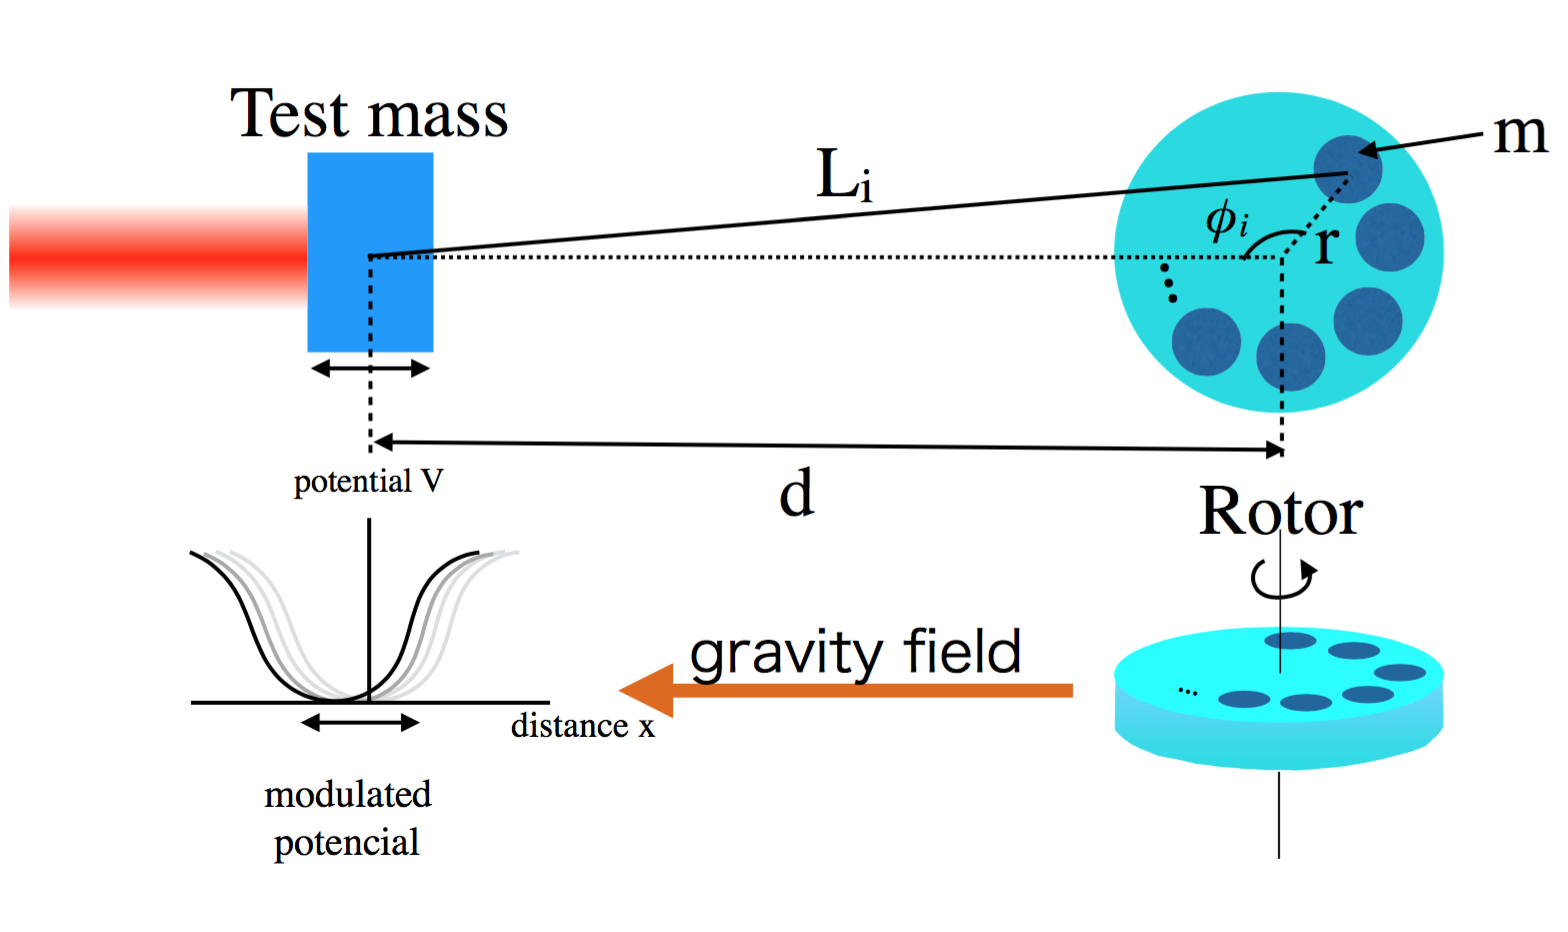
\includegraphics[width=12cm]{dim.eps}
\caption{}
\label{fig:dim}
\end{center}
\end{figure}

Distance between i-th mass and center of test mass is 
\begin{equation}
L_i=d \sqrt{1+\left( \frac{r}{d} \right)^2 -2\left( \frac{r}{d} \right) \cos{\phi_i} },
\end{equation}
where the angle of i-th mass is assumed as $\phi_i=\omega_{rot} t + 2\pi i/N$.
The gravity potential at the center of test mass can be described as
\begin{eqnarray}
V &=& \Sigma^N_{i=0} V_i \\
&=&-\frac{GMm}{d} \Sigma^N_{i=0} \Sigma^{\infty}_{n=0} \left( \frac{r}{d} \right)^n P_n\left(\cos{\left(\omega_{rot} t +\frac{2 \pi i}{N}\right)}\right),
\end{eqnarray}
where $P_n$ is Legendre polynomial. The equation of motion of test mass is 
\begin{equation}
Ma=\left| \frac{\partial V}{\partial{d}} \right| =\frac{GMm}{d^2}\Sigma^N_{i=0} \Sigma^{\infty}_{n=0}(n+1) \left( \frac{r}{d} \right)^n P_n\left(\cos{\left(\omega_{rot} t +\frac{2 \pi i}{N}\right)}\right),
\end{equation}
where $a$ is acceleration of test mass. We place the quadrupole and hexapole masses in same rotor as shown in Fig.~\ref{frg:hex}. We will calculate the displacement of quadrupole and hexapole in the section ~\ref{Quad} 

\begin{figure}
\begin{center}
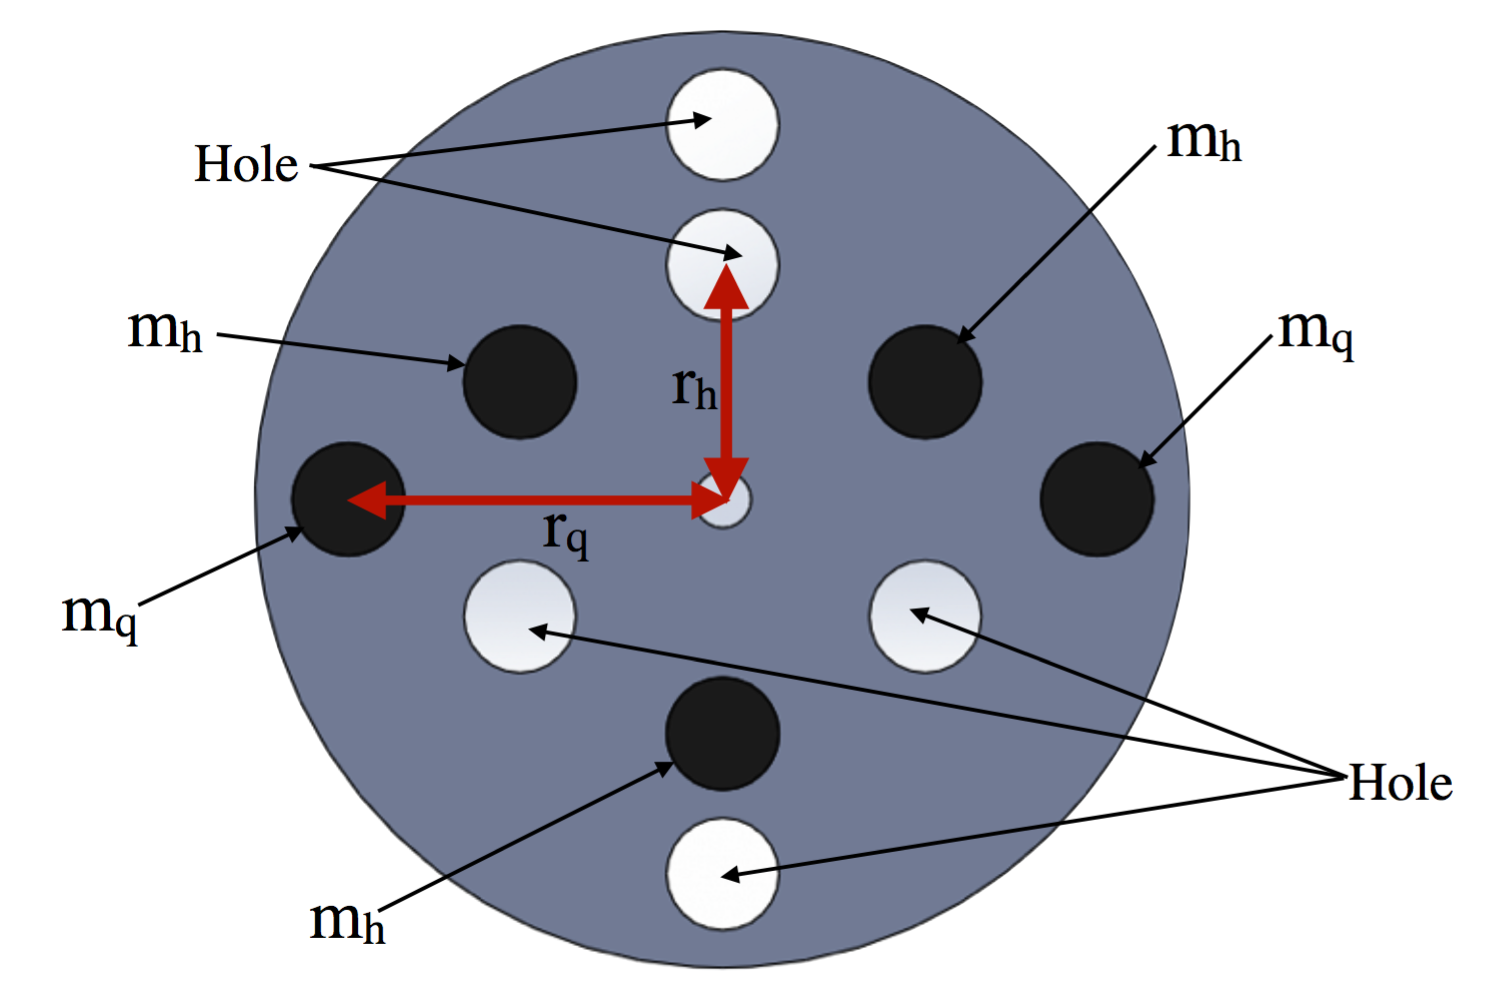
\includegraphics[width=12cm]{Hexapole.eps}
\caption{}
\label{fig:hex}
\end{center}
\end{figure}

\subsection{Displacement of test mass(Quadrupole)} \label{Quad}
We calculate the displacement of the quadrupole mass distribution, which corresponds to $N=2$.
The mass and radius of quadrupole are assumed as $m_q$, $r_q$. 
The equation of motion of test mass is described as
\begin{equation}
Ma=\frac{GMm_q}{d^2}\Sigma^{\infty}_{n=0}(n+1) \left( \frac{r_q}{d} \right)^n \left( P_n\left(\cos{\left(\omega_{rot} t \right)}\right) + P_n\left(\cos{\left(\omega_{rot} t +\pi \right)}\right) \right).
\end{equation} 
If we assume $r \ll d$, the displacement of the time-dependent lower harmonics can be written by 
\begin{equation}
x=\Sigma_{i=1}^{\infty}x_{n\mathrm{f}}\cos(n\omega_{rot} t)\sim x_{2\mathrm{f}}\cos(2\omega_{rot} t)=x_{2f}\cos{\omega t},
\end{equation}
where amplitude of 2-f is
\begin{equation}
x_{2\mathrm{f}}=\frac{9}{8}\frac{GMm_{q}r_{q}^2}{d^4}s(\omega). \label{2f}
\end{equation}

\subsection{Displacement of test mass(Haxapole)} \label{Hexa}
We calculate the displacement of the quadrupole mass distribution, which corresponds to $N=3$.
The mass and radius of quadrupole are assumed as $m_h$, $r_h$. 
The equation of motion of test mass is described as
\begin{eqnarray}
Ma = \frac{GMm_h}{d^2}\Sigma^{\infty}_{n=0}(n+1) \left( \frac{r_h}{d} \right)^n \\
\times \left( P_n\left(\cos{\left(\omega_{rot} t \right)}\right) + P_n\left(\cos{\left(\omega_{rot} t+\frac{2\pi}{3} \right)} \right) + P_n\left(\cos{\left(\omega_{rot} t \frac{4\pi}{3} \right) }\right) \right).
\end{eqnarray} 
If we assume $r \ll d$, the displacement of the time-dependent lower harmonics can be written by 
\begin{equation}
x=\Sigma_{i=1}^{\infty}x_{n\mathrm{f}}\cos(n\omega_{rot} t)\sim  x_{3\mathrm{f}}\cos(3\omega_{rot} t)=x_{3f}\cos{\omega t},
\end{equation}
where amplitude of 3-f is
\begin{equation}
 x_{3\mathrm{f}}=\frac{5}{6}\frac{GMm_{h}r_{h}^3}{d^5}s(\omega). \label{3f}
\end{equation}

\section{Absolute power calibration by using Gcal and Pcal}
In this section, we will discuss about absolute laser power calibration using interferometer. 
Figure~\ref{fig:IFO} shows the configuration of absolute laser power calibration.
First, we modulate the mirror position using gravity field calibrator. We can measure the peaks of $x_{2f}$ and $x_{3f}$ in the response o interferometer. Second, we send the interferometer signal to the excitation port of photon calibrator as a reference and performs feedback control. Third, we measure the absolute laser power at the detector of transmitter module and receiver module. By using Eq~(\ref{pcal}),(\ref{2f}), and (\ref{3f}), the modulated powers are
\begin{eqnarray}
 P_{2f}=\frac{9}{4} \frac{Gcm_{q}Mr_{q}^2}{d^4cos\theta}\frac{1}{1+\frac{M}{I}\vec{a}\cdot \vec{b}} \label{2f} \\
 P_{3f}= \frac{5}{3} \frac{Gcm_{h}Mr_{h}^3}{d^5cos\theta}\frac{1}{1+\frac{M}{I}\vec{a}\cdot \vec{b}} \label{3f}
\end{eqnarray}
Fourth, we demodulate the signal of transmitter module and receiver module using the encoder signal of gravity field calibrator.
The demodulated signals are 
\begin{eqnarray}
V_{2f}^{T}=\rho_{T}P_{2f} \\
V_{2f}^{R}=\rho_{R}P_{2f} \\
V_{3f}^{T}=\rho_{T}P_{3f} \\
V_{3f}^{R}=\rho_{R}P_{3f} 
\end{eqnarray} 
Therefore, we can estimate the distance using measured data. 
\begin{equation}
d=\frac{20}{27} \frac{V_{2f}^T}{V_{3f}^T}\frac{m_{h}}{m_{q}}\frac{r_{h}^{3}}{r_{q}^{2}}=\frac{20}{27} \frac{V_{2f}^R}{V_{3f}^R}\frac{m_{h}}{m_{q}}\frac{r_{h}^{3}}{r_{q}^{2}} \label{d}
\end{equation}
Using Eq (\ref{d}),(\ref{2f}) and (\ref{3f}), we can calibrate the absolute leaser power.

\begin{figure}
\begin{center}
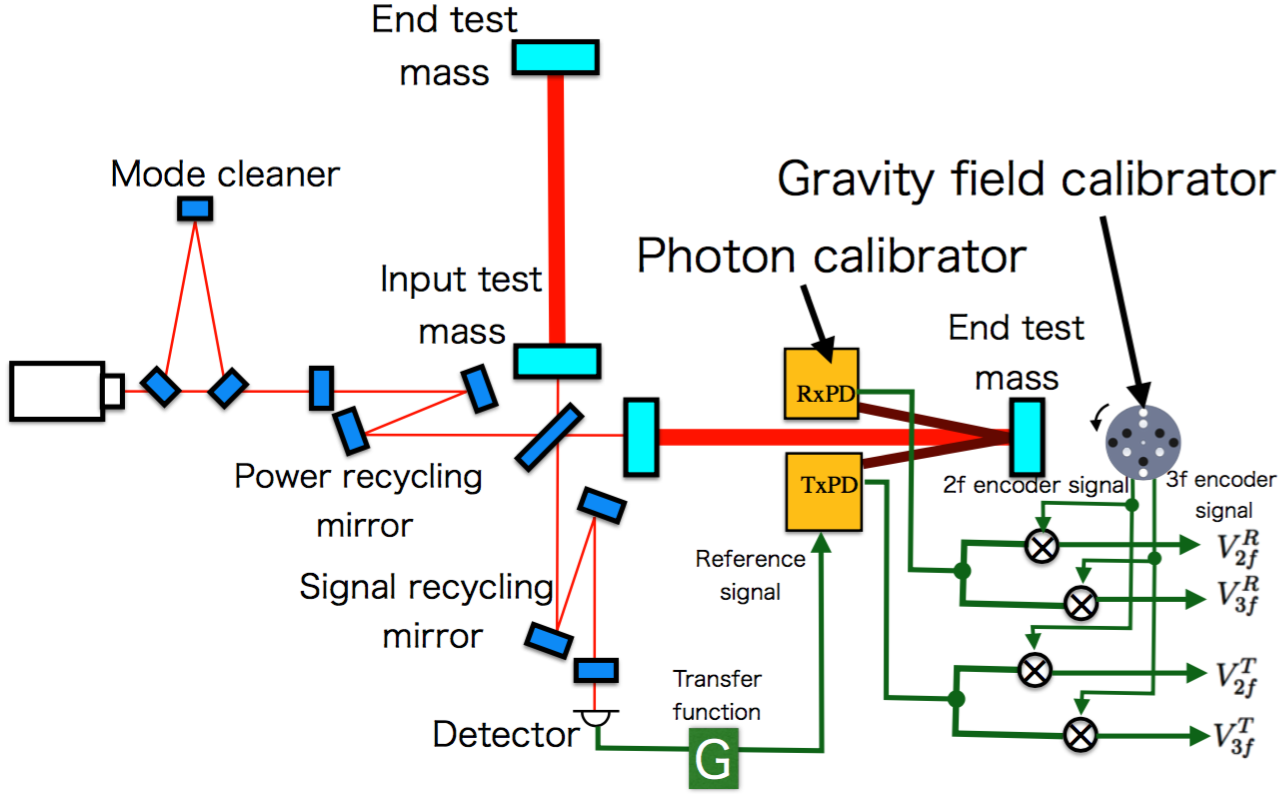
\includegraphics[width=12cm]{IFO.eps}
\caption{}
\label{fig:IFO}
\end{center}
\end{figure}

\section{Estimation of uncertainty}
We estimate the uncertainty of laser power. The assumed parameters are listed in Table XXX. (13)と(14)についてのエラーをモンテカルロで計算する

\begin{figure}
\begin{center}
\includegraphics[width=12cm]{peaks.eps}
\caption{}
\label{fig:peaks}
\end{center}
\end{figure}

\begin{table}
\begin{center}
\caption{\label{sus}The assumed parameters.}
\footnotesize
\begin{tabular}{ccc}
\br
$G$& Gravity constant&\\
$c$& speed of light[m/sec]&\\
$I$& Inertia[$\mathrm{kg m^2}$]&\\
$\theta$& Incident andgle[deg]&0.7\\
$M$& Mass of test mass[kg]&23\\
$m_q$&Mass of quadrupole[kg]&3.777\\
$m_h$&Mass of hexapole[kg]& 7.404\\
$r_q$&Radius of quadrupole[m]&0.130\\
$r_h$&Radius of hexapole[m]& 0.060\\
$d$&Distance[m]& 2.00\\
\br
\end{tabular}\\
\end{center}
\end{table}

\section{Discussion}
伝達関数がキャンセルする利点こと。低い周波数だとIMの効果を入れないといけなく、伝達関数のズレがあること。反跳効果と追随効果。
いつでも絶対キャリブレーションができること。
窓の効果率や積分球の効果を介さず計算できること。
r/dの数字によっては、1%の効果を考えるときにルジャンドル多項式の高次の効果を入れないといけない。有限要素法との比較。
ローターのパラメータのオプティマイズ。

\section{Summary}


\begin{verbatim}

\end{verbatim}



\end{document}

